\chapter{Análise espacial: Fundamentos}

\pagestyle{fancy}

A análise espacial é uma das tarefas fundamentais, sem a qual o conceito de SIG não atinge seu verdadeiro potencial.

A análise espacial é o \textbf{estudo quantitativo dos fenômenos que se manifestam no espaço}. Isso envolve aspectos cruciais como posição, área, distância e interação espacial.

Fora de um SIG, exemplos de análise espacial incluem: localizar o pico mais alto em um mapa, verificar a altitude de uma cidade, ou planejar uma rota turística considerando distância, tempo e melhores estradas. Todas essas ações são exemplos de análise geográfica — que também podem ser feitas em um SIG.

Através da análise, podemos gerar novos dados como \textbf{camadas geográficas, tabelas, valores escalares} ou \textbf{vetores}.

Às vezes o resultado expressa \textbf{a mesma variável} dos dados de origem (como a média), outras vezes, \textbf{a variável de entrada e saída são diferentes} (por exemplo, gerar uma camada de declividade a partir de uma de elevação).

A análise espacial pode combinar \textbf{diferentes tipos de dados}, como elevação + localização urbana = média de altitude da cidade. Em SIG, seriam duas camadas combinadas no processo.

A análise em SIG permite formular e responder a questões como:

\begin{itemize}
 \item Relacionadas à \textbf{posição e extensão}
 \item Relacionadas à \textbf{forma e distribuição}
 \item Relacionadas à \textbf{associação espacial}
 \item Relacionadas à \textbf{interação espacial}
 \item Relacionadas à \textbf{variação espacial}
\end{itemize}

\section{Exemplos de análise espacial}

\subsection{Consulta espacial}

Consultas, já vistas no capítulo de bancos de dados, podem ser integradas a outras análises — como seleção prévia de entidades a serem analisadas.

\subsection{Análise topológica}

Permite consultas baseadas em \textbf{relações entre elementos}, por exemplo:

\begin{itemize}
 \item Qual o caminho mais curto da minha posição até determinado ponto?
 \item Quais estados fazem fronteira com São Paulo?
\end{itemize}

\subsection{Medições}

Com a referência espacial, é possível \textbf{quantificar}:

\begin{itemize}
 \item Distâncias, áreas, perímetros, índices de forma
 \item Declividade, orientação, índices derivados
\end{itemize}

\subsection{Combinação de camadas}

Combinar ou \textbf{sobrepor camadas} é uma das operações mais características dos SIG.

No caso de camadas vetoriais, são comuns operações como \textbf{união, interseção, diferença e recorte}. Ver Figura~\ref{Fig:Interseccion}.

\begin{figure}[!hbt]   
\centering
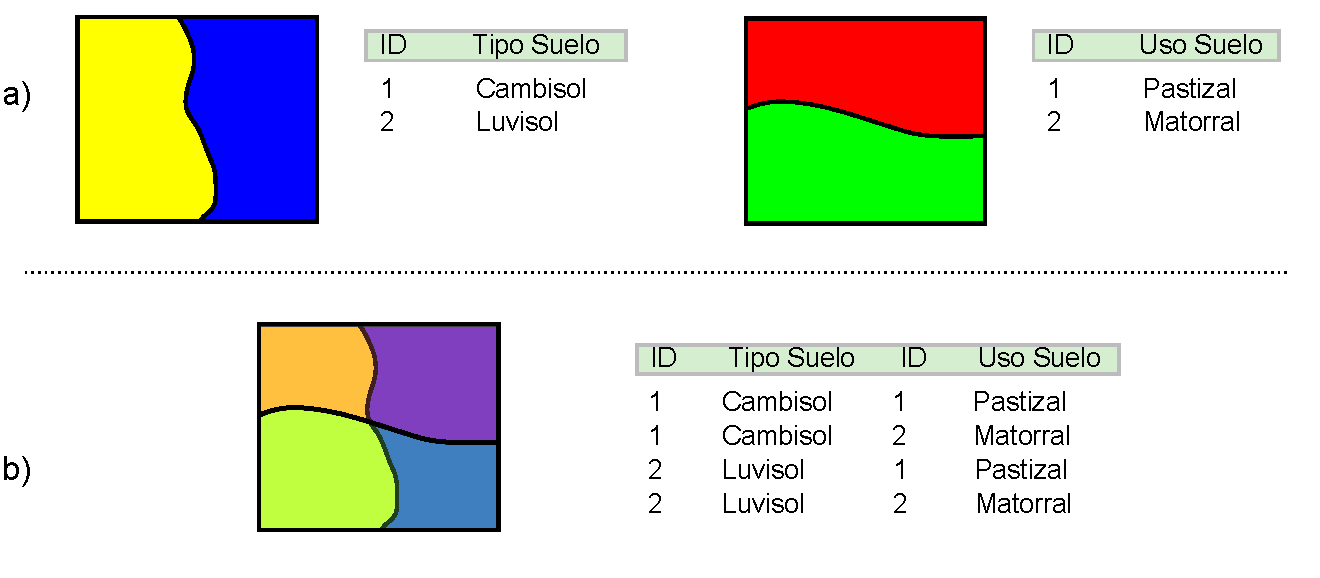
\includegraphics[width= \columnwidth]{Analises/Interseccion.pdf}
\caption{\small Interseção de duas camadas de polígonos.}
\label{Fig:Interseccion} 
\end{figure}

\subsection{Transformações}

Incluem processos como:

\begin{itemize}
 \item \textbf{Transformação de coordenadas}
 \item \textbf{Simplificação de geometria}
 \item \textbf{Áreas de influência}
 \item \textbf{Reclassificação de valores}
 \item \textbf{Conversão entre modelos raster e vetorial}
\end{itemize}

Ver Figura~\ref{Fig:Conversiones} para exemplo de conversão de curvas de nível (vetorial) para MDE (raster).

\begin{figure}[!hbt]   
\centering
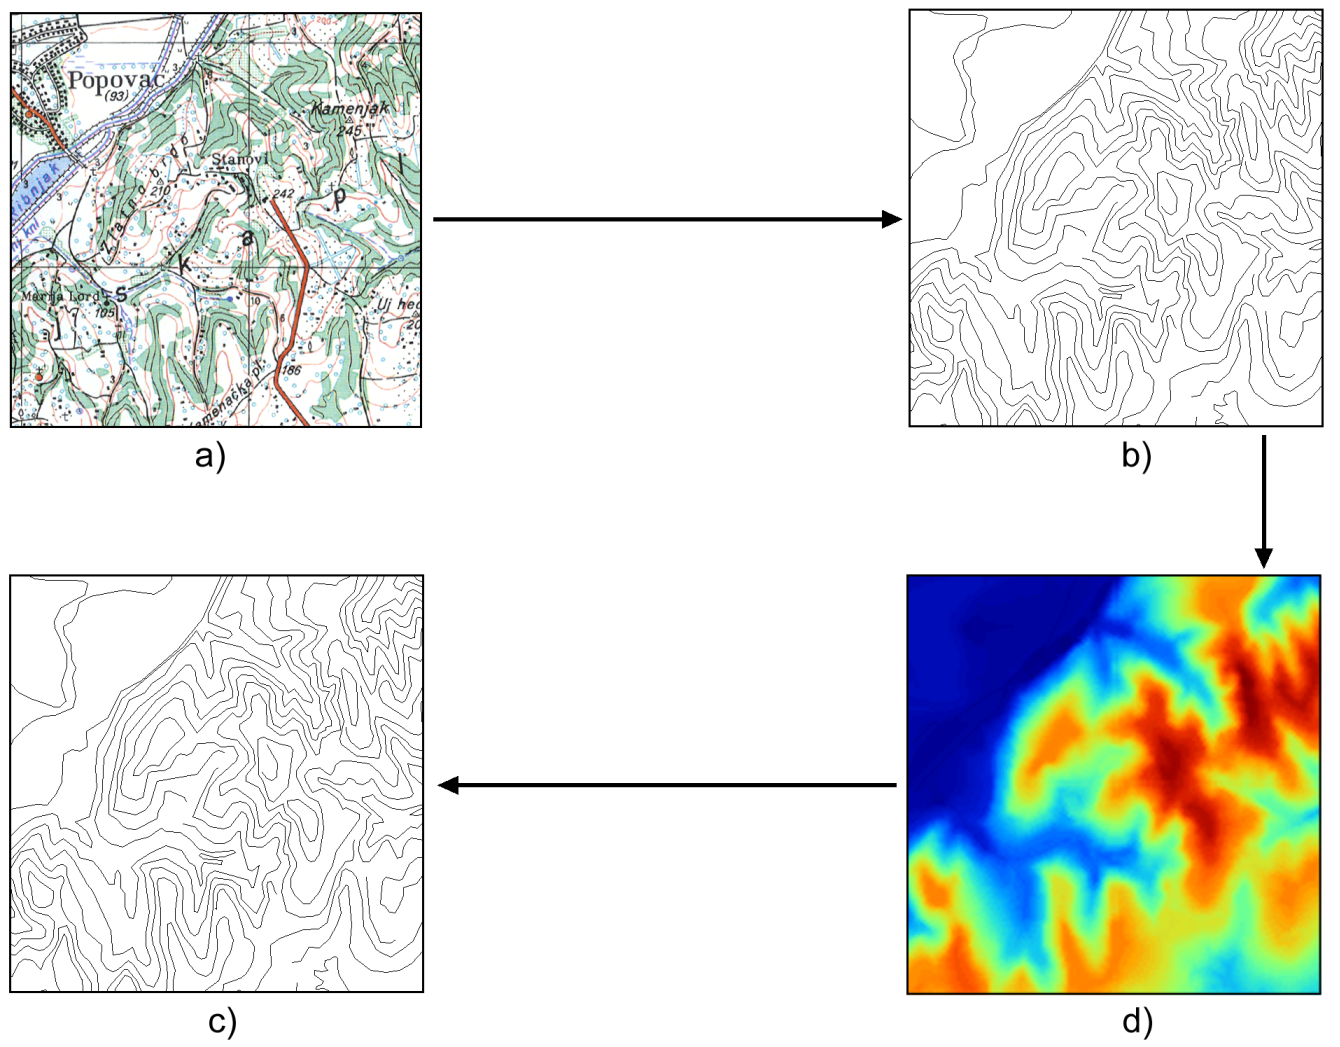
\includegraphics[width= \columnwidth]{Analises/Conversiones.png}
\caption{\small Conversão entre modelos de dados para uma camada de elevação.}
\label{Fig:Conversiones} 
\end{figure}

\subsection{Análise de superfícies}

Inclui:

\begin{itemize}
 \item \textbf{Declividade}, \textbf{orientação}
 \item Análises morfométricas
 \item \textbf{Modelagem hidrológica}
\end{itemize}

\subsection{Estatística descritiva}

Permite avaliar os dados espacialmente com:

\begin{itemize}
 \item Média, mediana, variância
 \item Dependência espacial
 \item Padrões espaciais
\end{itemize}

Exemplos:

\begin{itemize}
 \item A altura média é constante no país?
 \item Há direção predominante nos deslocamentos de uma espécie?
\end{itemize}

\subsection{Inferência}

Utilizada para \textbf{modelar comportamento e prever evolução} espacial ao longo do tempo. Fundamental para análises de mudança e tendência.

\subsection{Tomada de decisão e otimização}

Permite cruzar múltiplos fatores:

\begin{itemize}
 \item Onde construir com menor impacto ambiental?
 \item Onde posicionar um hospital para atender melhor a população?
\end{itemize}

\subsection{Modelagem}

Modelos espaciais são cada vez mais viáveis em SIG — pela estrutura de dados e possibilidade de automação de processos.

\section{Particularidades dos dados espaciais na análise}

\subsection{Escala}

Além da escala cartográfica, existe a \textbf{escala de análise}, que depende dos dados e do tipo de estudo.

Ver Figura~\ref{Fig:Escalas_formas_terreno} — um ponto pode ser uma colina ou fundo de vale dependendo da escala.

\begin{figure}[h]   
\centering
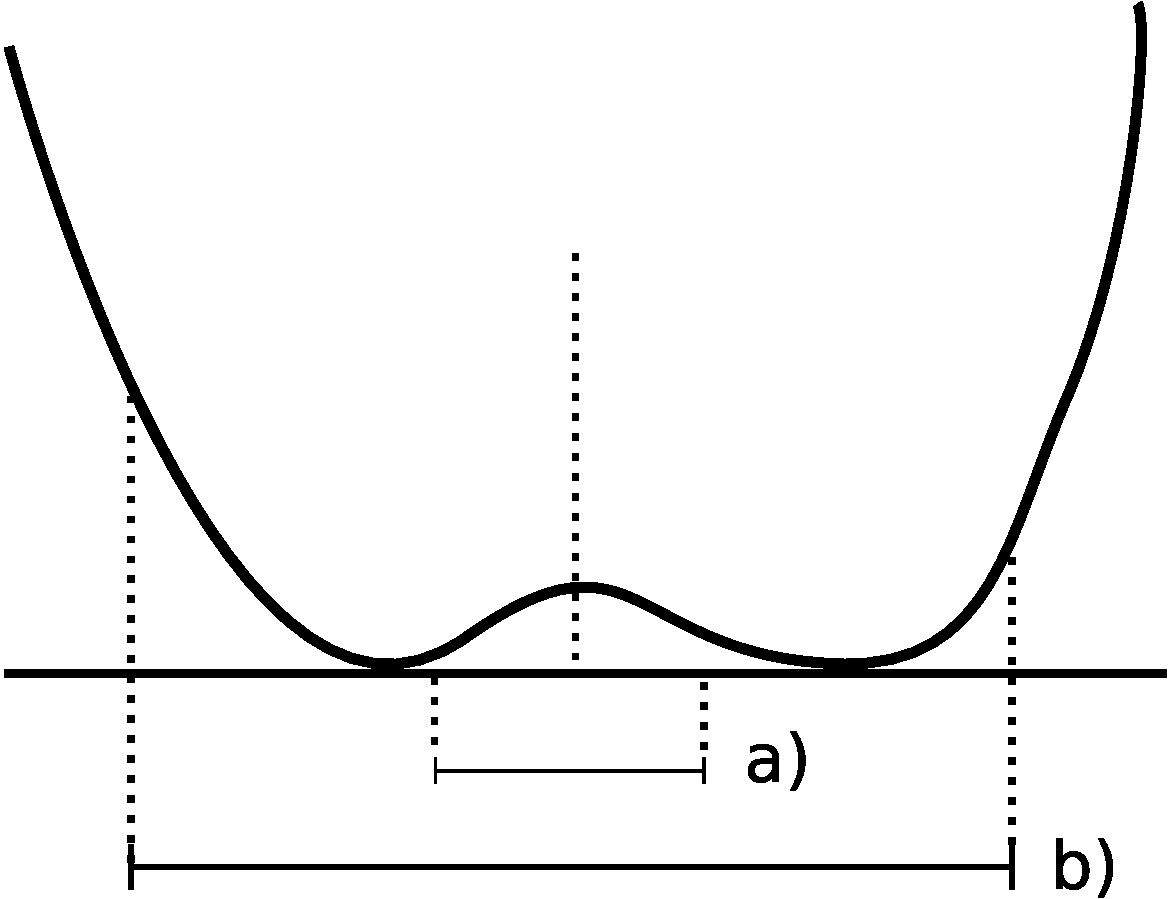
\includegraphics[width= .45\columnwidth]{Analises/Escalas_formas_terreno.pdf}
\caption{\small Um mesmo ponto pode ser identificado como cume (a) ou vale (b), dependendo da escala.}
\label{Fig:Escalas_formas_terreno} 
\end{figure}

Também se aplica à \textbf{medição de comprimentos}, como mostra a Figura~\ref{Fig:Medida_linea_fractal}.

\begin{figure}[h]   
\centering
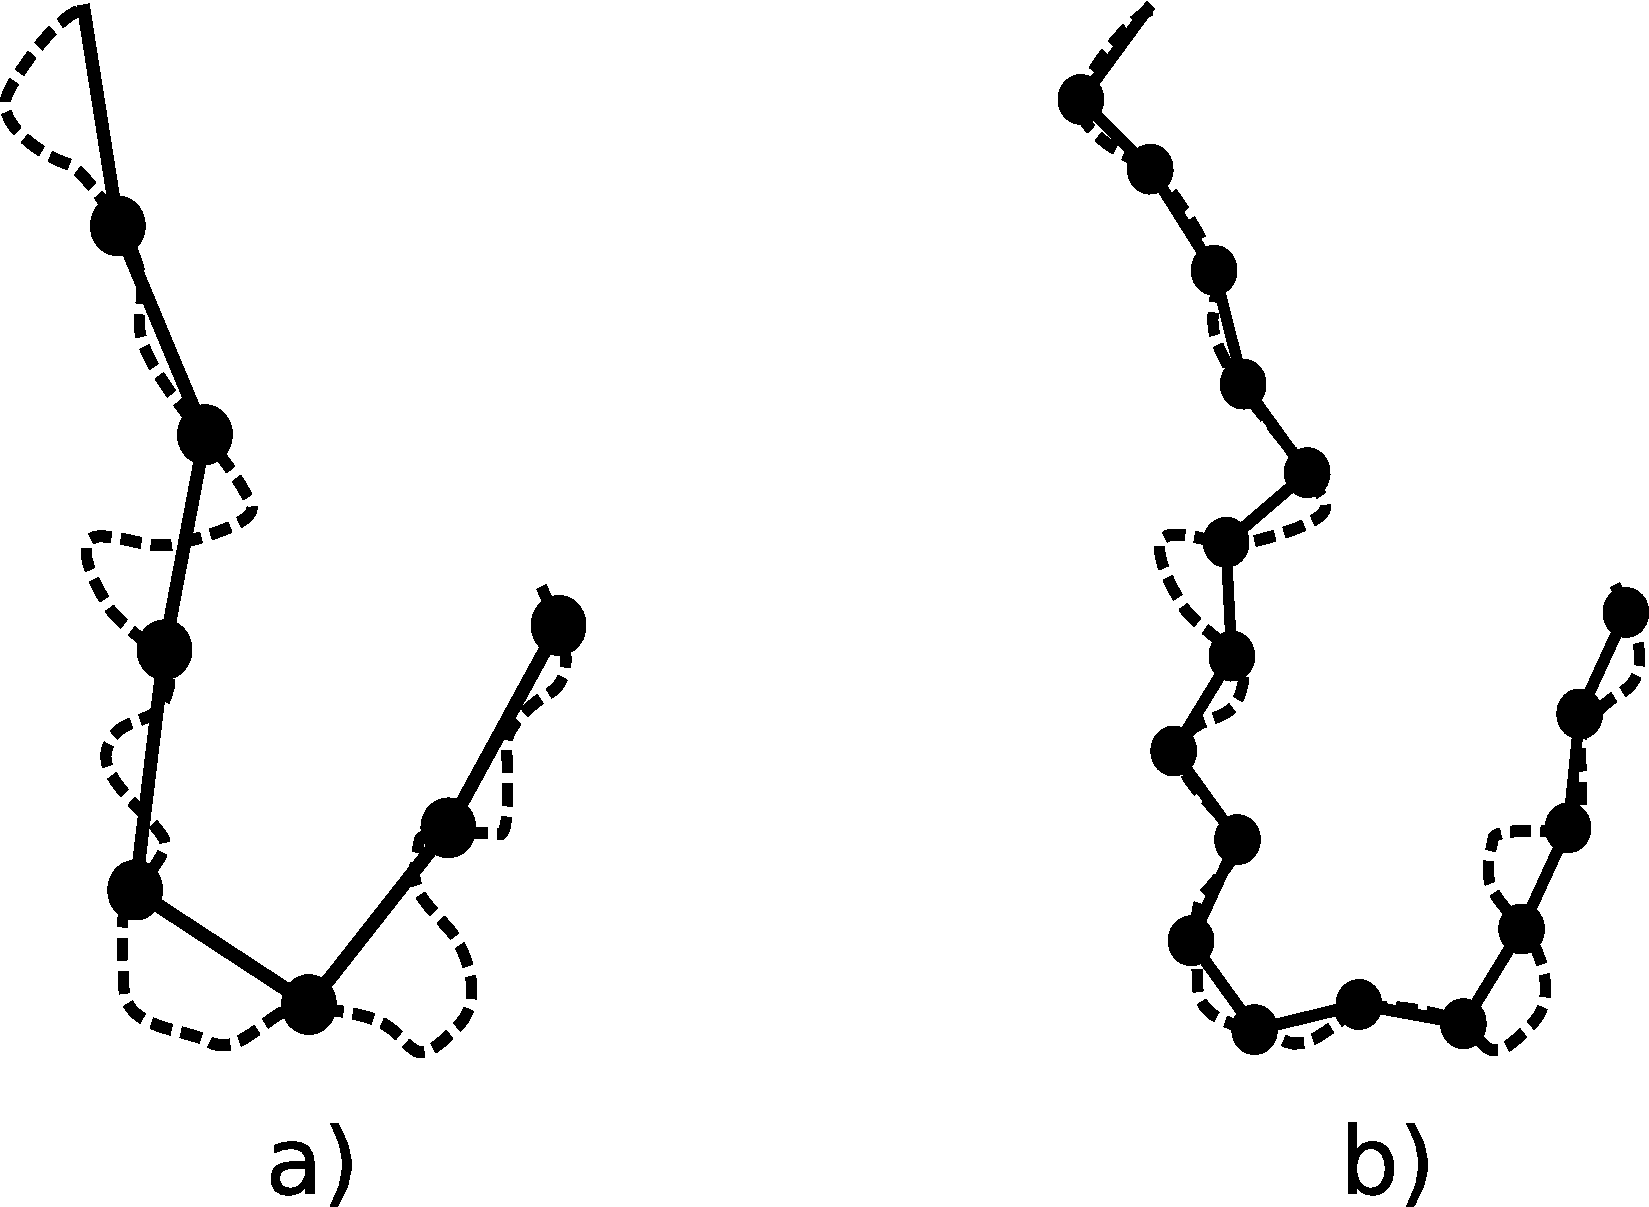
\includegraphics[width= .45\columnwidth]{Analises/Medida_linea_fractal.pdf}
\caption{\small O comprimento medido depende da unidade usada.}
\label{Fig:Medida_linea_fractal} 
\end{figure}

Isso está diretamente ligado ao conceito de \textbf{fractal}.

O \textbf{formato de dados} também limita a escala — ex: \textbf{tamanho da célula} em dados raster.

\subsection{Problema da Unidade de Área Modificável (PUAM)}

Algumas variáveis (ex: densidade populacional) não são pontuais, mas calculadas por área.

As unidades usadas (distritos, municípios) são arbitrárias e \textbf{afetam os resultados}. Isso é o PUAM.

Relacionado a isso, temos a \textbf{falácia ecológica}: assumir que os dados médios de uma área valem para todos os indivíduos nela contidos.

\subsection{Autocorrelação espacial}

É a \textbf{correlação de uma variável consigo mesma no espaço}. Pode ser:

\begin{itemize}
 \item \textbf{Positiva} — valores semelhantes próximos (temperatura)
 \item \textbf{Negativa} — valores opostos próximos
 \item \textbf{Inexistente} — valores independentes no espaço
\end{itemize}

Ver Figura~\ref{Fig:Autocorrelacion_espacial}.

\begin{figure}[!hbt]   
\centering
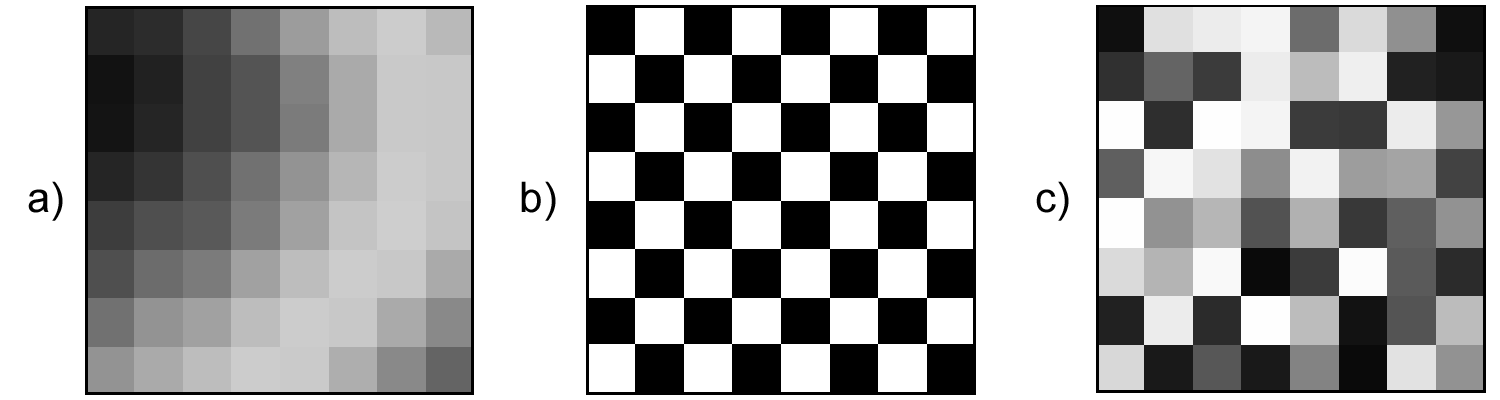
\includegraphics[width=\textwidth]{Analises/Autocorrelacion_espacial.png}
\caption{\small a) Positiva, b) Negativa, c) Sem correlação espacial.}
\label{Fig:Autocorrelacion_espacial} 
\end{figure}

A autocorrelação viola suposições estatísticas de independência. Deve ser considerada nos modelos. Porém, pode ser usada para \textbf{interpolação}.

\subsection{Estrutura dos dados espaciais}

Dois conceitos definem a estrutura espacial:

\begin{itemize}
 \item \textbf{Estacionaridade} — invariância por translação (sem tendência espacial)
 \item \textbf{Isotropia} — invariância por rotação (mesmo comportamento em todas as direções)
\end{itemize}

\subsection{Efeitos de borda}

Limites artificiais ou naturais distorcem análises, especialmente em parâmetros que dependem de área (ex: densidade).

Além disso, o \textbf{efeito pode se propagar} — elementos conectados ao limite também são afetados, mesmo se estiverem longe.

\pagestyle{empty}
